
% to choose your degree
% please un-comment just one of the following
\documentclass[bsc,frontabs,twoside,singlespacing,parskip,deptreport]{infthesis}     % for BSc, BEng etc.
% \documentclass[minf,frontabs,twoside,singlespacing,parskip,deptreport]{infthesis}  % for MInf
\usepackage{todonotes}
\usepackage{hyperref}

\begin{document}


\title{CoStor, a peer-to-peer distributed backup solution}

\author{Robert Phipps}

\course{Computer Science}
\project{4th Year Project Report}

\date{\today}

\abstract{
This is an example of {\tt infthesis} style.
The file {\tt skeleton.tex} generates this document and can be 
used to get a ``skeleton'' for your thesis.
The abstract should summarise your report and fit in the space on the 
first page.
%
You may, of course, use any other software to write your report,
as long as you follow the same style. That means: producing a title
page as given here, and including a table of contents and bibliography.
}

\maketitle

\section*{Acknowledgements}
This project makes extensive use and builds on top of concepts explored in this paper from
Paul Anderson and Le Zhang: Fast and secure laptop backups with encrypted de-duplication
\cite{macbac-lisa}

\tableofcontents

%\pagenumbering{arabic}


\chapter{Solution overview}

CoStor is designed as a turnkey solution to the problem of maintaining reliable system
backups within an SME with multiple sites, such as a confederation of schools. Instead
of using expensive and bandwidth intensive cloud storage services for offsite backup, 
CoStor is designed to hold a complete local backup on-site within the CoStor server, as
well as automatically replicating backup data across a group of federated instances of
the server software, ensuring that there is always at least two redundant copies of the
backup datastore in two different physical locations.

To simplify networking requirements for deployment, all communication between clients 
and servers, both locally and between sites, makes use of standard HTTPS requests. This 
negates the need for complex multi-site VPNs, and simply requires a single TCP port to
be forwarded to the server from the internet.

The backup datastore's metadata and directory structures are maintained inside an SQL
database and can only be modified over the RESTful HTTP API, reducing attack surface
compared to making use of more traditional file transfer methods like FTP, NFS or 
SSHFS.

All management is completed through a simple web UI, where clients can be configured 
for one-touch deployment and subsequently monitored, as well as where users can browse
the directory trees for each backup "snapshot" in the event that a file needs to be
recovered. A full backup restore can be completed by requesting a restoration archive,
whereby the server will build a complete archive of a snapshot, pulling data from its
local datastore, or from other sites in the event of a remote restore.

This system makes use of Django for server-side components, a Python web framework with
fantastic ORM and enforcement of best-practices.

\clearpage

\section{Goals of CoStor}

Given the target organisations for CoStor, there are some specific goals that need to be 
targeted during development.

\begin{itemize}
	\item \textbf{Reliable backups}
		\subitem As should be very obvious, being a backup solution, CoStor needs to be
		able to reliably manage and maintain backups for a network. This includes
		protections such as an "append-only" API for backup clients, validation of 
		uploaded data, and mitigations against the most common reasons a backup
		may be called upon such as accidental deletion, user errors, hardware failure and 
		ransomware style attacks.
	\item \textbf{Simple restores}
		\subitem As this system is targeted at small organisations which may not have their
		own full-time IT support staff, restoring from backups should be straightforward 
		for an end-user. This is achieved through the use of a self-service web UI.
	\item \textbf{Robust security and audit logs}
		\subitem Backups almost always contain confidential information, so CoStor needs 
		to be able to manage permissions on a granular user-by-user basis. It also needs 
		to include audit logging for all operations on the system. Any offsite storage and
		"data in flight" needs to be strongly encrypted to protect confidentiality.
	\item \textbf{Low maintenance}
		\subitem Systems tend to be forgotten about, and in the case of backups, often you
		only notice something hasn't been working once you need to restore 
		something\footnote{GitLab found this to their cost in 2017 after discovering their 
		backups hadn't been running for some time: 
		\url{https://techcrunch.com/2017/02/01/gitlab-suffers-major-backup-failure-after-data-deletion-incident/}},
		so CoStor needs to include built in maintenance and scheduled self-tests to ensure
		that the system is ready when the user needs it most.
	\item \textbf{Simple deployment}
		\subitem Again, CoStor needs to be deployable by inexperienced IT support staff
		without prior knowledge of network filesystems, command line interfaces or web
		development. This can be achieved by making use of clever packaging and deployment 
		strategies such as Docker for server components and zero-touch installation scripts
		for backup clients. By making use of standard and well understood protocols such
		as HTTP(S) for communication between components, compatibility with most network
		architectures should be maintained, without the requirement for complex network 
		share configurations, multi-site VPNs and authentication systems.
	\item \textbf{Centralised management and monitoring}
		\subitem As this is designed to be deployed over a large number of client PCs,
		ensuring configuration is correct could be challenging. As such, CoStor will include
		configuration of backup clients from the server management panel, and all clients
		will pull down configuration automatically from this central repository. Backup
		logs will also be pushed to the server so that an administrator can monitor their
		entire estate from a single place.
	\item \textbf{Distributed and fault-tolerant file stores}
		\subitem Leaving the best to last, CoStor's standout feature will be that backups
		can be automatically replicated between federated instances of the CoStor server, 
		over a zero-configuration HTTPS link. The system should be able to recover from the
		loss of a server without any data loss, and allow restoration of data originating
		from any site from any of the remaining instances of CoStor within the network.
\end{itemize}

\section{Limitation of scope for the purposes of this project}

As this project is to completed by an individual over the course of a single academic year, 
the scope does unfortunately have to be limited somewhat. The primary goal is to complete
a "Beta" release of the server application, with cross-site replication, web UI and ability
to restore data, along with a barebones backup client to allow the system to be demonstrated.

Managing filesystem metadata and ensuring consistent snapshots is a considerable problem in its
own right.

\clearpage

\section{Exploration of existing solutions}

There are many packages in existence which incorporate a subset of the features targeted
by this project, however most either focus on the synchronisation features with some 
limited support for file history, and no robust backup capability, whereas others rely on
cloud storage infrastructure as the backend, distributed datastore which either necessitates
the use of a commercial provider such as AWS S3\footnote{Amazon Web Services' bucket 
storage solution} or BackBlaze B2. Both of these greatly increase cost and introduce a 
reliance on a third party.

A number of existing products have been selected as they offer the closest functionality
to that targeted by CoStor, and are explored here:

\subsection{Syncthing}

Syncthing is a service targeted at consumers who want a self-hosted alternative to commercial
cloud storage and synchronisation services such as Dropbox, Google Drive and OneDrive. The 
agent software can be configured to sync any file changes between two or more devices, allowing
for access anywhere, with a form of georeplication. It also requires fairly minimal network
configuration, just needing a pair of ports to be opened on at least one of the nodes to allow
discovery of other agents.

A very large distinction has to be made in the fact that "Syncthing is a continuous file 
synchronization program"\cite{syncthing}, in that it isn't designed to create restorable 
snapshots of your data, and therefore is completely unsuitable for robust \textit{backup} of 
important information.

More information is available at \url{https://syncthing.net} \cite{syncthing}

\subsection{UrBackup}

UrBackup is closer to CoStor in its goals, as is specifically built to be used as a backup 
system. It can auto-discover agents on the network, and begin incremental backups to its server
software. It also supports full image backups of NTFS formatted drives with bare metal 
restore. UrBackup has many of the features targeted by CoStor, including a simple web interface
for management, however it does not include any built-in support for georeplication.

More information is available at \url{https://www.urbackup.org/index.html} \cite{urbackup}

\subsection{Hermes}

Hermes is an "open-source redundant distributed storage network"\cite{hermes}. Although it
doesn't come pre-packaged with components allowing it to be used as a turnkey backup system,
it is worth exploring as it does specifically target the geo-replication features for the 
purposes of backup that CoStor is looking to integrate. It promises fast, encrypted and seamless
replication and sharding of data across nodes in the network, making use of LZMA compression
to increase performance.

This would appear to be a very promising option to integrate as the backend storage for CoStor,
however it looks like the project is very much stale, with the last commits being made in late 
2014. As such, its codebase is somewhat limited in utility, given its lack of ongoing 
maintenance. It is also written in Go, with limited documentation, which is not a language
that I am familiar enough with to begin work on reviving.

More information is available at \url{https://github.com/Hermes/hermes} \cite{hermes}

\subsection{Bacula}

Bacula is an open-source and very mature backup framework, with tools to allow a multitude of
network configurations. Unfortunately its flexibilty does result in the software being complex
to configure. CoStor is targeting small organisations with limited in-house IT support capacity,
so this would likely be too complex to deploy without the assistance of external contractors. 
Bacula is also available in an "enterprise" edition\cite{bacula-ent}, which includes 
support as part of the subscription cost, however this version is both closed-source and
not inconsiderably expensive.

More information is available at \url{https://www.bacula.org} \cite{bacula}

\subsection{Amanda}

Amanda is another backup-specific solution, again with a "community edition" being accompanied
by a commercially supported "enterprise" version of the software. Like the other systems 
investigated, it targets backup to local storage, NAS drives and traditional tape backup
libraries, so would not be suitable for the use case targeted by CoStor.

More information is available at \url{https://www.zmanda.com/amanda-community-edition.html} \cite{zmanda}

\subsection{GlusterFS}

The Gluster filesystem is a "software scalable network filesystem"\cite{gluster-home}, which 
allows systems administrators to build complex filesystems across multiple physical machines
using commodity hardware. Gluster is targeted at engineers designing private cloud environments
which need large volumes of storage accessible from many devices, and has a huge number of 
configuration options to allow, among other things, redundant replicated storage across machines.
It also has support for filesystem filters that can offer encryption at a filesystem level before
data is transmitted between nodes.

Unfortunately for CoStor's usecase, this system is built on the assumption that the Gluster 
volumes are configured at the point of deployment, by the same user on all sites. It also is
primarily managed through a command line interface, with limited Python bindings, and is targeted
at an architecture where all nodes have rights to see data within the volume. Finally, it is
based around a master-slave architecture, which is unsuitable if CoStor were to be using a shared
volume for all nodes. It would be possible to wrangle a Gluster configuration to match what is
required by CoStor, where each site has its own volume, with its own georeplication session, 
however this would be very difficult to automatically provision from the CoStor web interface, 
and should be mostly unnecessary given the data structure used for backups.

More information is available at \url{https://www.gluster.org} \cite{gluster-home}

\section{Deployment topology}

The basic topology of a CoStor network would be as follows:

\begin{itemize}
	\item \textbf{Clients} (many):
	\subitem The CoStor client software is installed on any systems which are to be backed up.
	It communicates over the local network to the site's local instance of the CoStor server.
	
	\item \textbf{Servers} (one per site/network):
	\subitem  There should be one instance of CoStor server on the internal private network of 
	any site that has clients to be backed up. There could be multiple instances running in one
	local network space, but they would operate as separate "sites" within the software. The 
	servers are the primary file store for a site, and manage replication between federated
	instances on other sites.
	
	\item \textbf{Federated servers} ($>2$ across multiple locations):
	\subitem These are additional instances of the server application, and can be on separate
	networks and in different physical locations. These communicate over the internet through
	a replication API to keep a redundant copy of all data from all servers. They can restore
	data from any site within the group in the event that a site's server fails, assuming the 
	target site's encryption key is provided.
\end{itemize}

\todo[inline]{TODO: Insert diagram of topology, and describe how data is distributed across the 
members of the CoStor network.}

\section{Specimen use case}

The initial inspiration for this project was a use case within a confederation of small, state
controlled schools. Each school currently spends a large amount of money on a third-party 
managed cloud backup solution - in the region of \pounds500 per year for only 20GB of backed
up data. This meant that they were unable to backup considerable portions of their data, leaving
some of their media based teaching resources vulnerable.

The purpose of the confederation is to allow the members to share resources and purchasing power
for resources that can be beneficial to all of them.

CoStor could be utilised by these schools to allow them to geo-replicate their backups among 
themselves, on commodity server hardware, allowing them to no longer be reliant on expensive
cloud backup solutions. Each site would have a single CoStor server appliance with their file
servers, databases, Microsoft Active Directory databases and any other critical data being
backed up by instances of CoStor client, allowing backups to complete rapidly across the high
speed LAN, with replication to other schools' CoStor servers being carried out overnight when 
the internet connection is quiet.

The system should be as close to turnkey and zero-maintenance as possible, allowing it to be
set up by their IT support contractors, and left to work for years at a time without much
interference.

\chapter{Client implementation}

\section{Summary}

CoStor clients are designed to be managed centrally through the CoStor server web interface,
therefore they require no GUI of their own, just a way to set the target server instance, 
required directory tree to backup (the backup root) and their authentication token. These are
set using a \texttt{.YAML} file, which is easy to push to clients with standard network 
management tools such as Microsoft Group Policy and Logon Scripts.

The client is built around Python 3, and PonyORM working in parallel with an SQlite database. 
This means there are very few dependencies, once the Python project is bundled, and allows
cross-platform development with a shared codebase.

\section{The backup process}

The backup process works as follows:

\begin{enumerate}
	\item \textbf{Build directory structure hashes}:
	The client uses the \texttt{HashTreeMaker} class to build a simplified version of the 
	directory tree being backed up, traversing through the tree bottom-up, and building objects
	for every item it encounters, each item identified by a hash based off of its attributes
	and the hashes of all its children. File data is also hashed and stored with a path to the
	file, to be used for backup later.
	
	\item \textbf{Local metadata database update}:
	The client keeps a local database of all backup "snapshots" as trees of objects, created by
	the hasher. It checks for an existing snapshot, and uses this to identify any subtrees within
	the backup root which have changed since the last backup run. It then writes any changes to
	the database as part of a new snapshot.
	
	\item \textbf{Authenticate with server}:
	A quick test is made to ensure that the client's credentials are valid and that the server is
	accessible.
	
	\item \textbf{Push changed metadata objects}:
	The server is queried to see if it has seen any objects with matching IDs (hashes), and any
	objects that are missing are pushed as a single JSON object.
	
	\item \textbf{File "primes" are pushed to the server}:
	Again, the server is queried to check for existing copies of any of the files that are 
	included in this backup snapshot, by hash. For any files that are missing, the client uses
	the path included with the object to find a copy of that file, and pushes it to the server,
	in multiple chunks.
\end{enumerate}

\section{Large file upload API}

To allow large files to be uploaded over standard HTTPS connections, with the ability to recover
from connection issues, files are split into (currently 100MB) chunks, which are individually
hashed, and then pushed in sequence to the server.

\begin{figure}[h]
	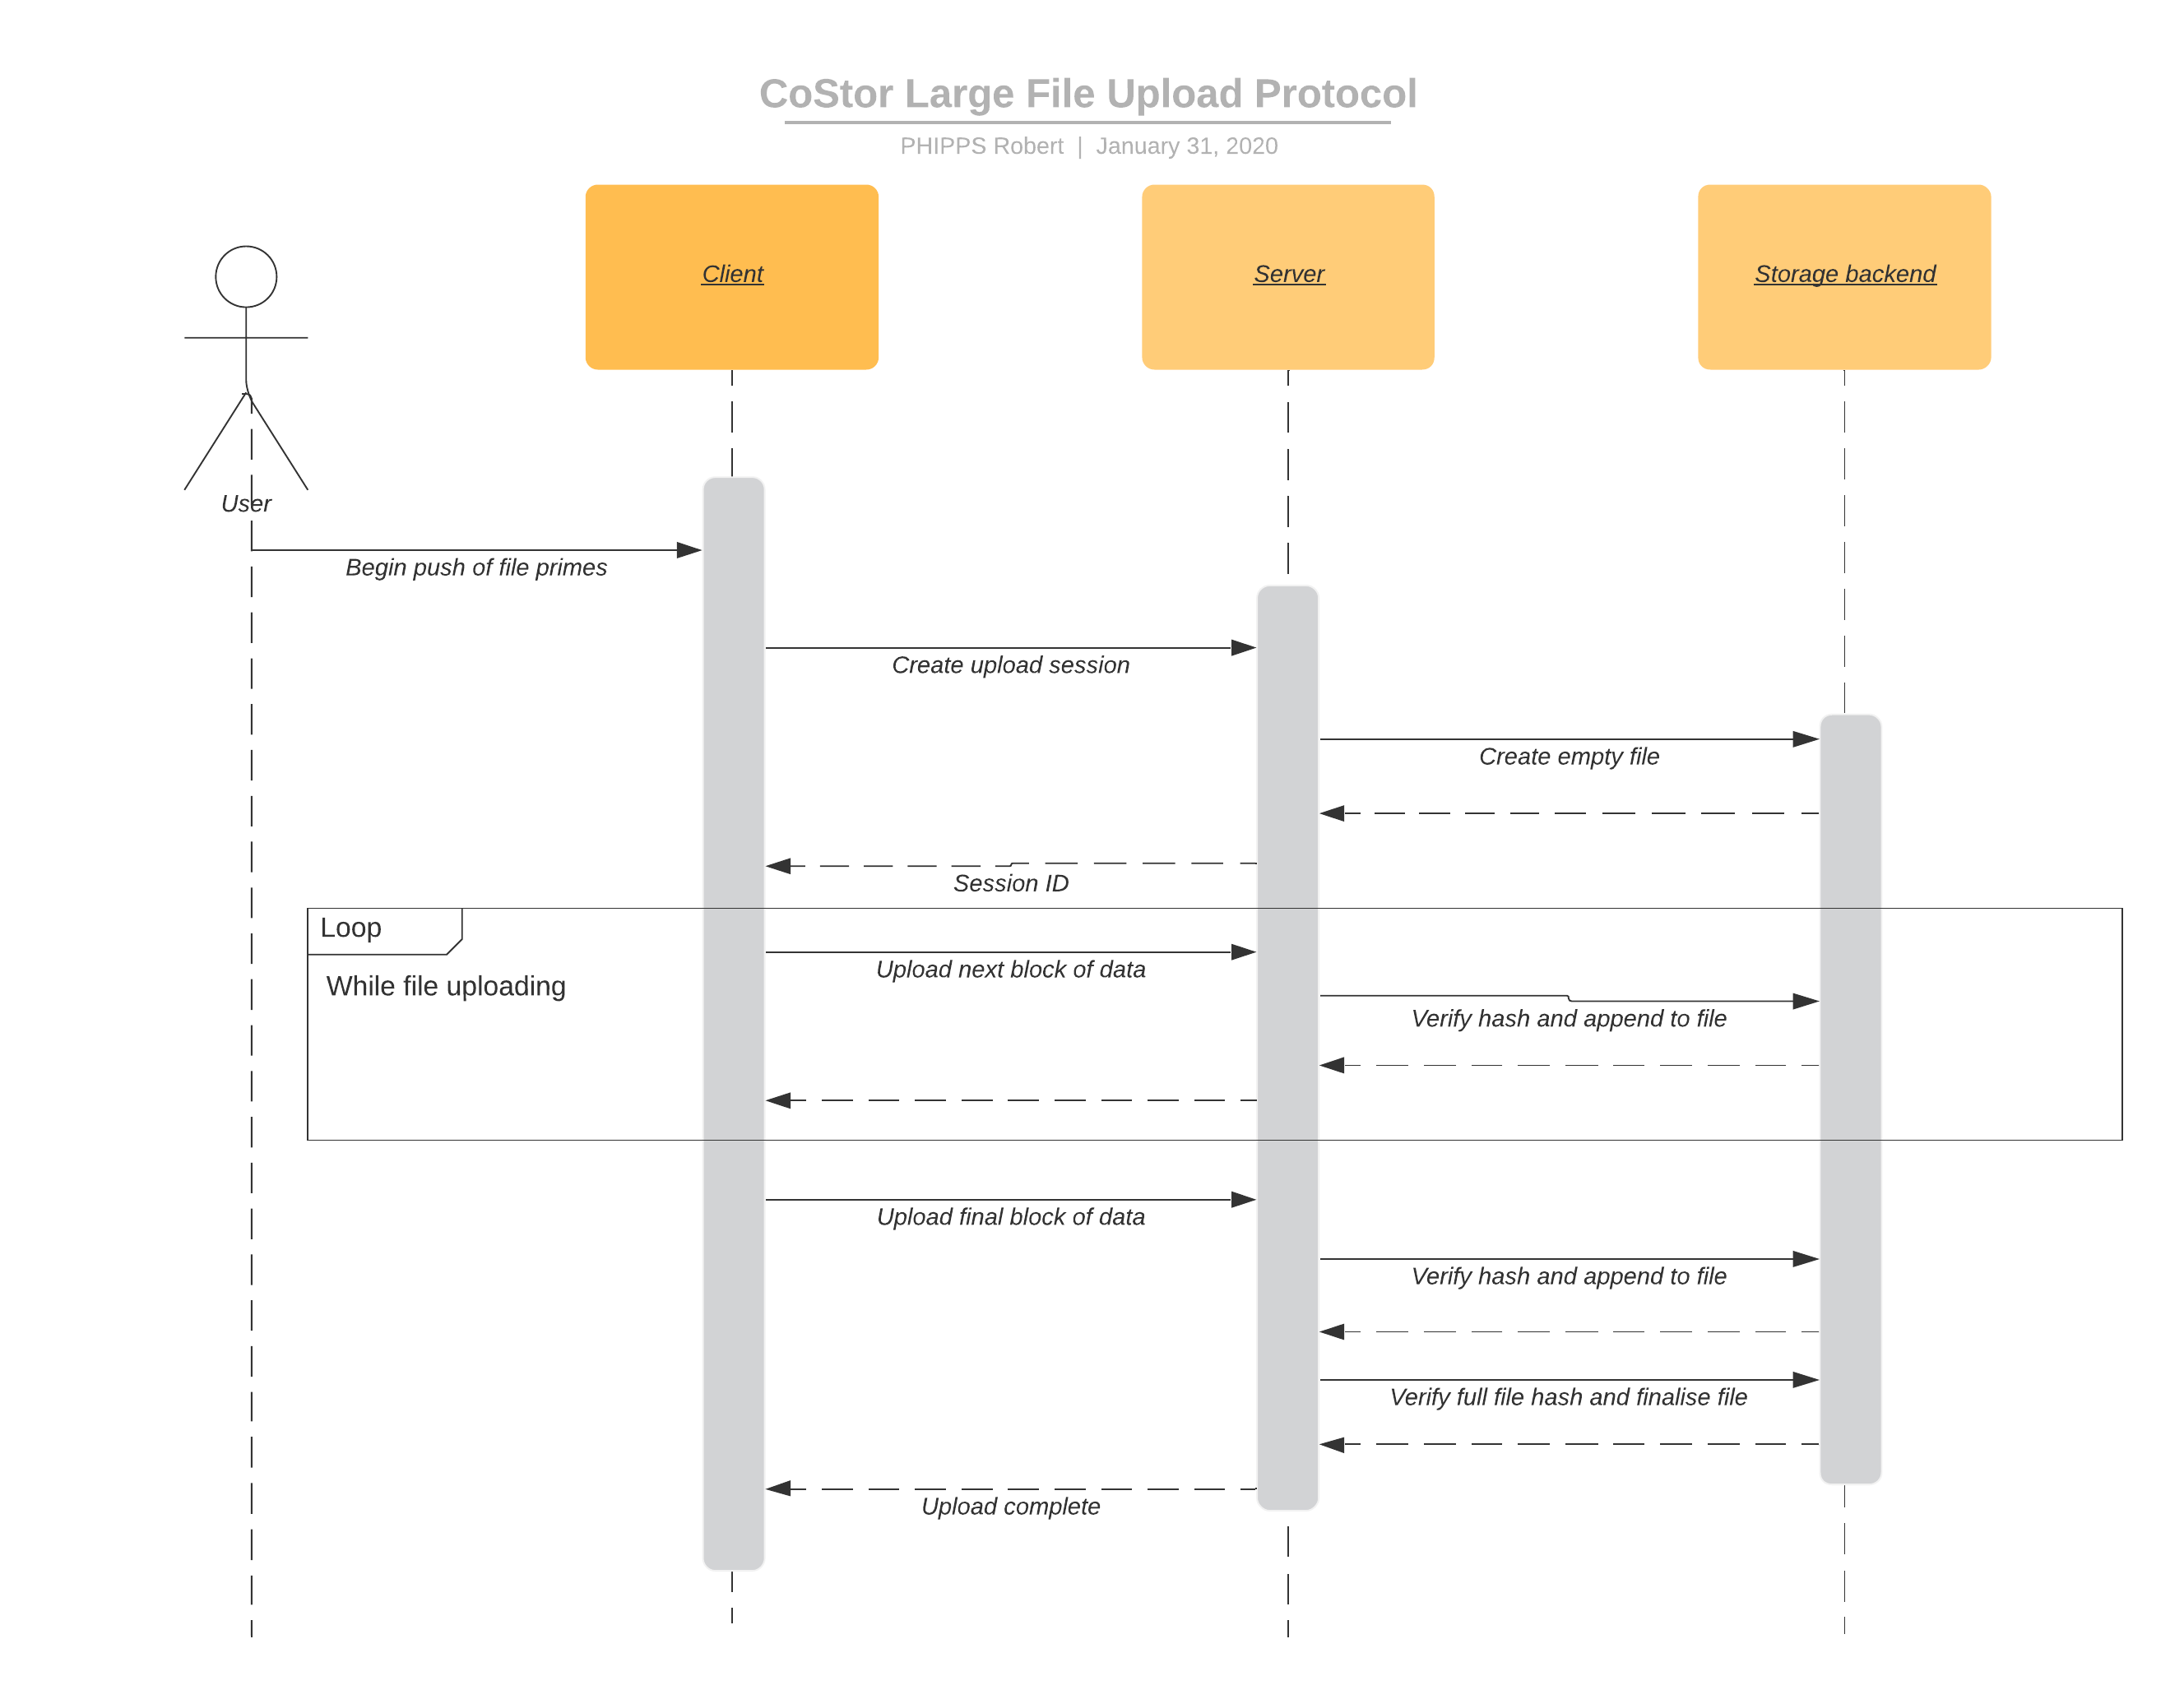
\includegraphics[width=\linewidth]{img/lfileupload.png}
	\caption{UML sequence diagram for large file upload}
	\label{fig:lfileupload}
\end{figure}

Integrity is ensured by having the client create an "upload session" before pushing chunks of
files. This session includes the file hash and the number of expected parts. Each part is also 
uploaded along with its hash and sequence number, which is verified before the data is appended 
to the file in the server's filesystem. Once the final part has been received, the server 
checks the completed file against the hash given in the upload session before marking the file
as complete and closing the session.

Chunks can be uploaded over any period of time, and chunks for one file/session can be uploaded
interspersed with chunks from other files, the only constraint is that chunks for a session are
received in correct sequence order.

Should a chunk fail its upload, due to a verification error or network instability, the client
is able to retry this chunk once network has been restored, allowing uploads to be "resumed", at 
least to the resolution of the chunk size.

\section{Management and monitoring}

\todo[inline]{Telemetry and configuration synchronisation is currently not implemented}

On each run, the client checks in with the server to pull down a configuration update, which 
includes chunk size, backup schedules, backup root, server version, and expiry time for local
metadata information. This allows it to ensure it is configured correctly, without needing local 
intervention from the administrator.

It also pushes up telemetry from backups including backup results and network speed statistics, 
as well as free disk space and local metadata database size.

\section{SQL database and other backup plugins}

\todo[inline]{Plugins are currently not implemented}

Included in the client are plugins to allow the client to automatically dump and backup common
applications such as Microsoft SQL Server. These plugins are simple Python modules installed in
the CoStor client install directory. Simple command line scripts can also be defined from the
CoStor server interface and pulled down with the client config package.

Current targeted software includes:

\begin{itemize}
	\item Microsoft SQL Server
	\item MySQL server (Windows/Linux)
	\item Microsoft Active Directory Server\footnote{https://docs.microsoft.com/en-us/windows/win32/ad/backing-up-an-active-directory-server}
\end{itemize}

\section{Filesystem snapshots and integrity protection}

\todo[inline]{The below has not yet been implemented}

To ensure that files cannot change during the backup process, it is necessary to create some form
of snapshot of the filesystem while the backup is running. This is currently being investigated
and will likely make use of LVM, Microsoft Shadow Copies and Time Machine on Linux, Windows and
MacOS respectively.

\section{The HashTreeMaker}

This class is the engine behind the creation of the filesystem metadata snapshot, and builds
simple objects that can be stored in the relational databases used by CoStor.

\begin{figure}[h]
	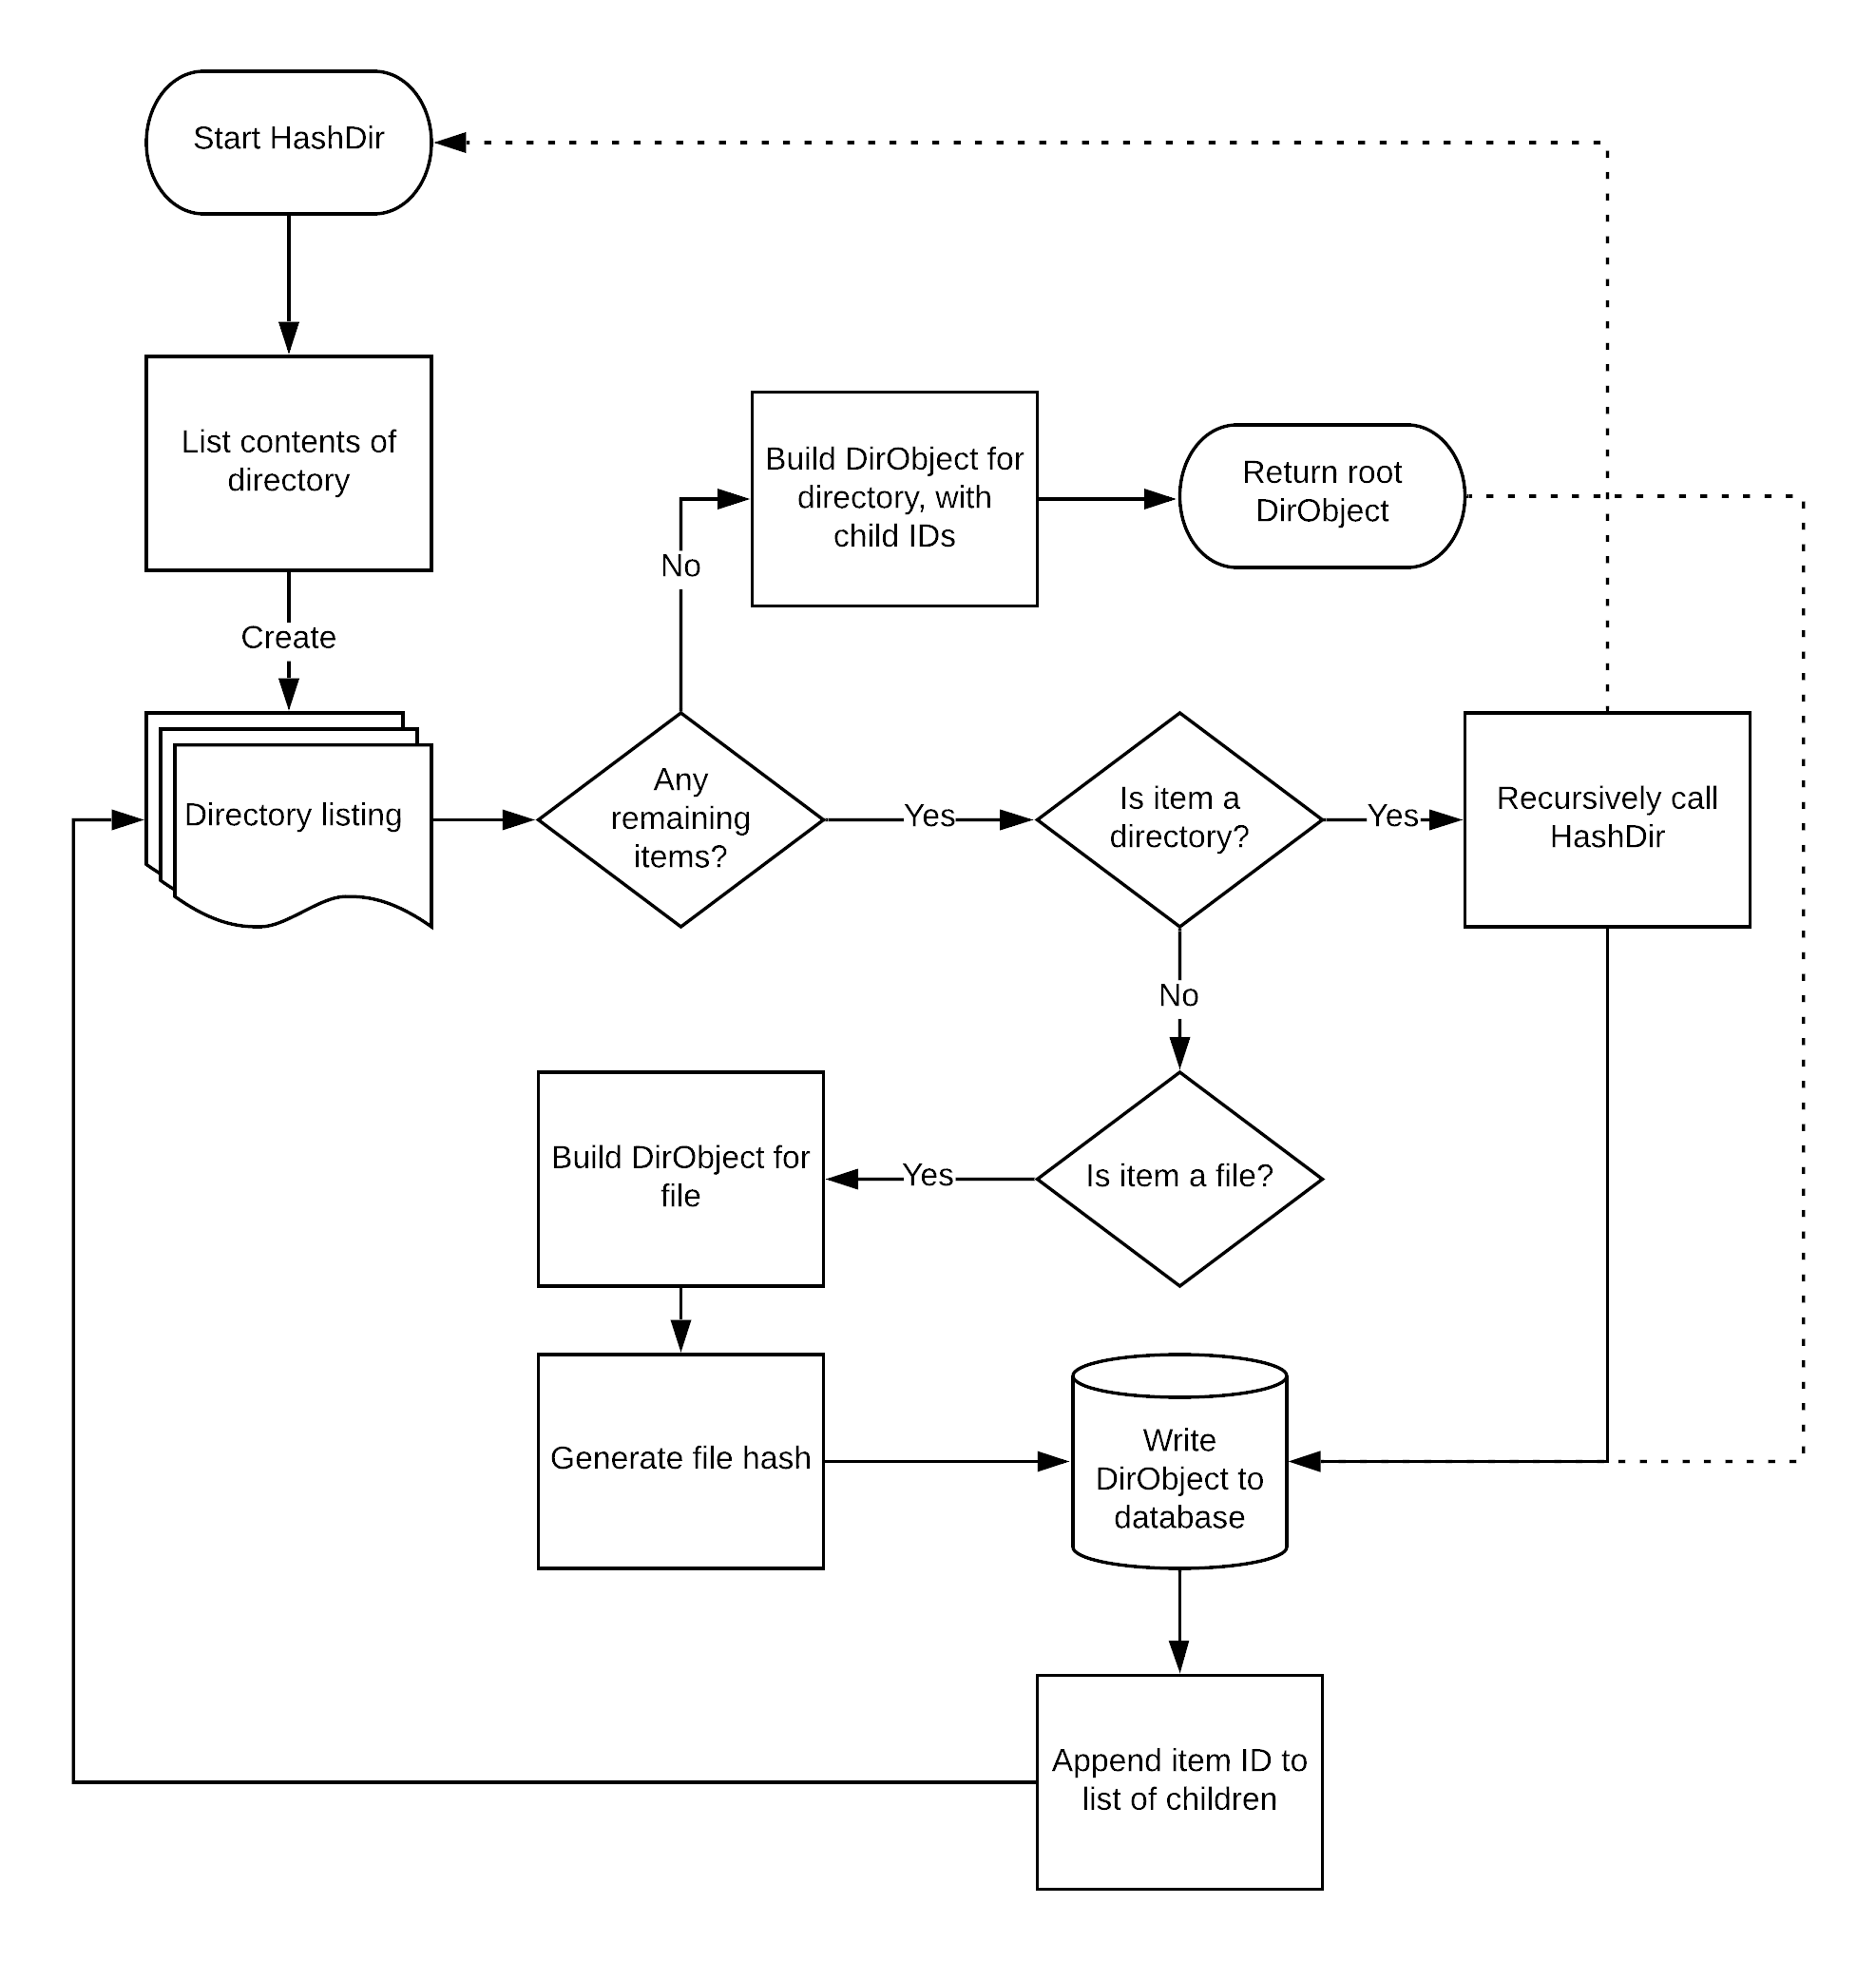
\includegraphics[width=\linewidth]{img/hasherflow.png}
	\caption{Process for creating DB representation of directory tree}
	\label{fig:hasherflow}
\end{figure}

\todo[inline]{This currently uses SHA1, which is not secure. TODO: move to BLAKE2}

\chapter{Server and datastore implementation}

\section{Current development status}

As of late January 2020, the CoStor server application is very minimal, simply accepting backups 
into its datastore, and all user interface is through the built in Django Admin pages API. As
standard model definitions are used, along with the Django REST Framework\footnote{\url{https://www.django-rest-framework.org}},
building API endpoints to expose this data to a custom front-end application should be incredibly
straightforward. Work to enable long-running and complex tasks is ongoing.

\section{Overview}

CoStor server is a Django based web application, that can be deployed within Docker for easy
installation and upgrades. It not only provides the backup API endpoints used by the Client
software to actually push snapshot data to the server's storage, but also a web UI for 
management and monitoring, as well as frameworks to allow replication of backup data between
instances of the server over a standard HTTPS connection.

To allow larger tasks (such as backup archive generation) to run asynchronously of the HTTP
requests to the web server, a task broker such as Celery\footnote{\url{http://www.celeryproject.org}} 
is used.

\clearpage

\section{High-level data architecture}

To allow all machinery to be as generalised as possible, all possible file system objects are stored
as generic \texttt{Object} objects. These can represent files, directories or symlinks. Each object
holds a globally unique ID, path information, the hash of the object's contents, child and parent 
relations, the path and link to a \texttt{DbFile} object or "prime" in the case that the object is
a file, with the prime representing the binary data of that file on the CoStor server's filesystem.

These objects are then related to their associated "snapshot" or backup session, backup root directory
and the agent (or CoStor client identity) that the backup originated from.

\section{Server metadata database and filestore}

All data on the CoStor server is stored within the context of the Django ORM, to allow easy access
to all objects using the powerful Object APIs provided by the ORM. The backup data is stored in the
following database models:

\begin{figure}[h]
	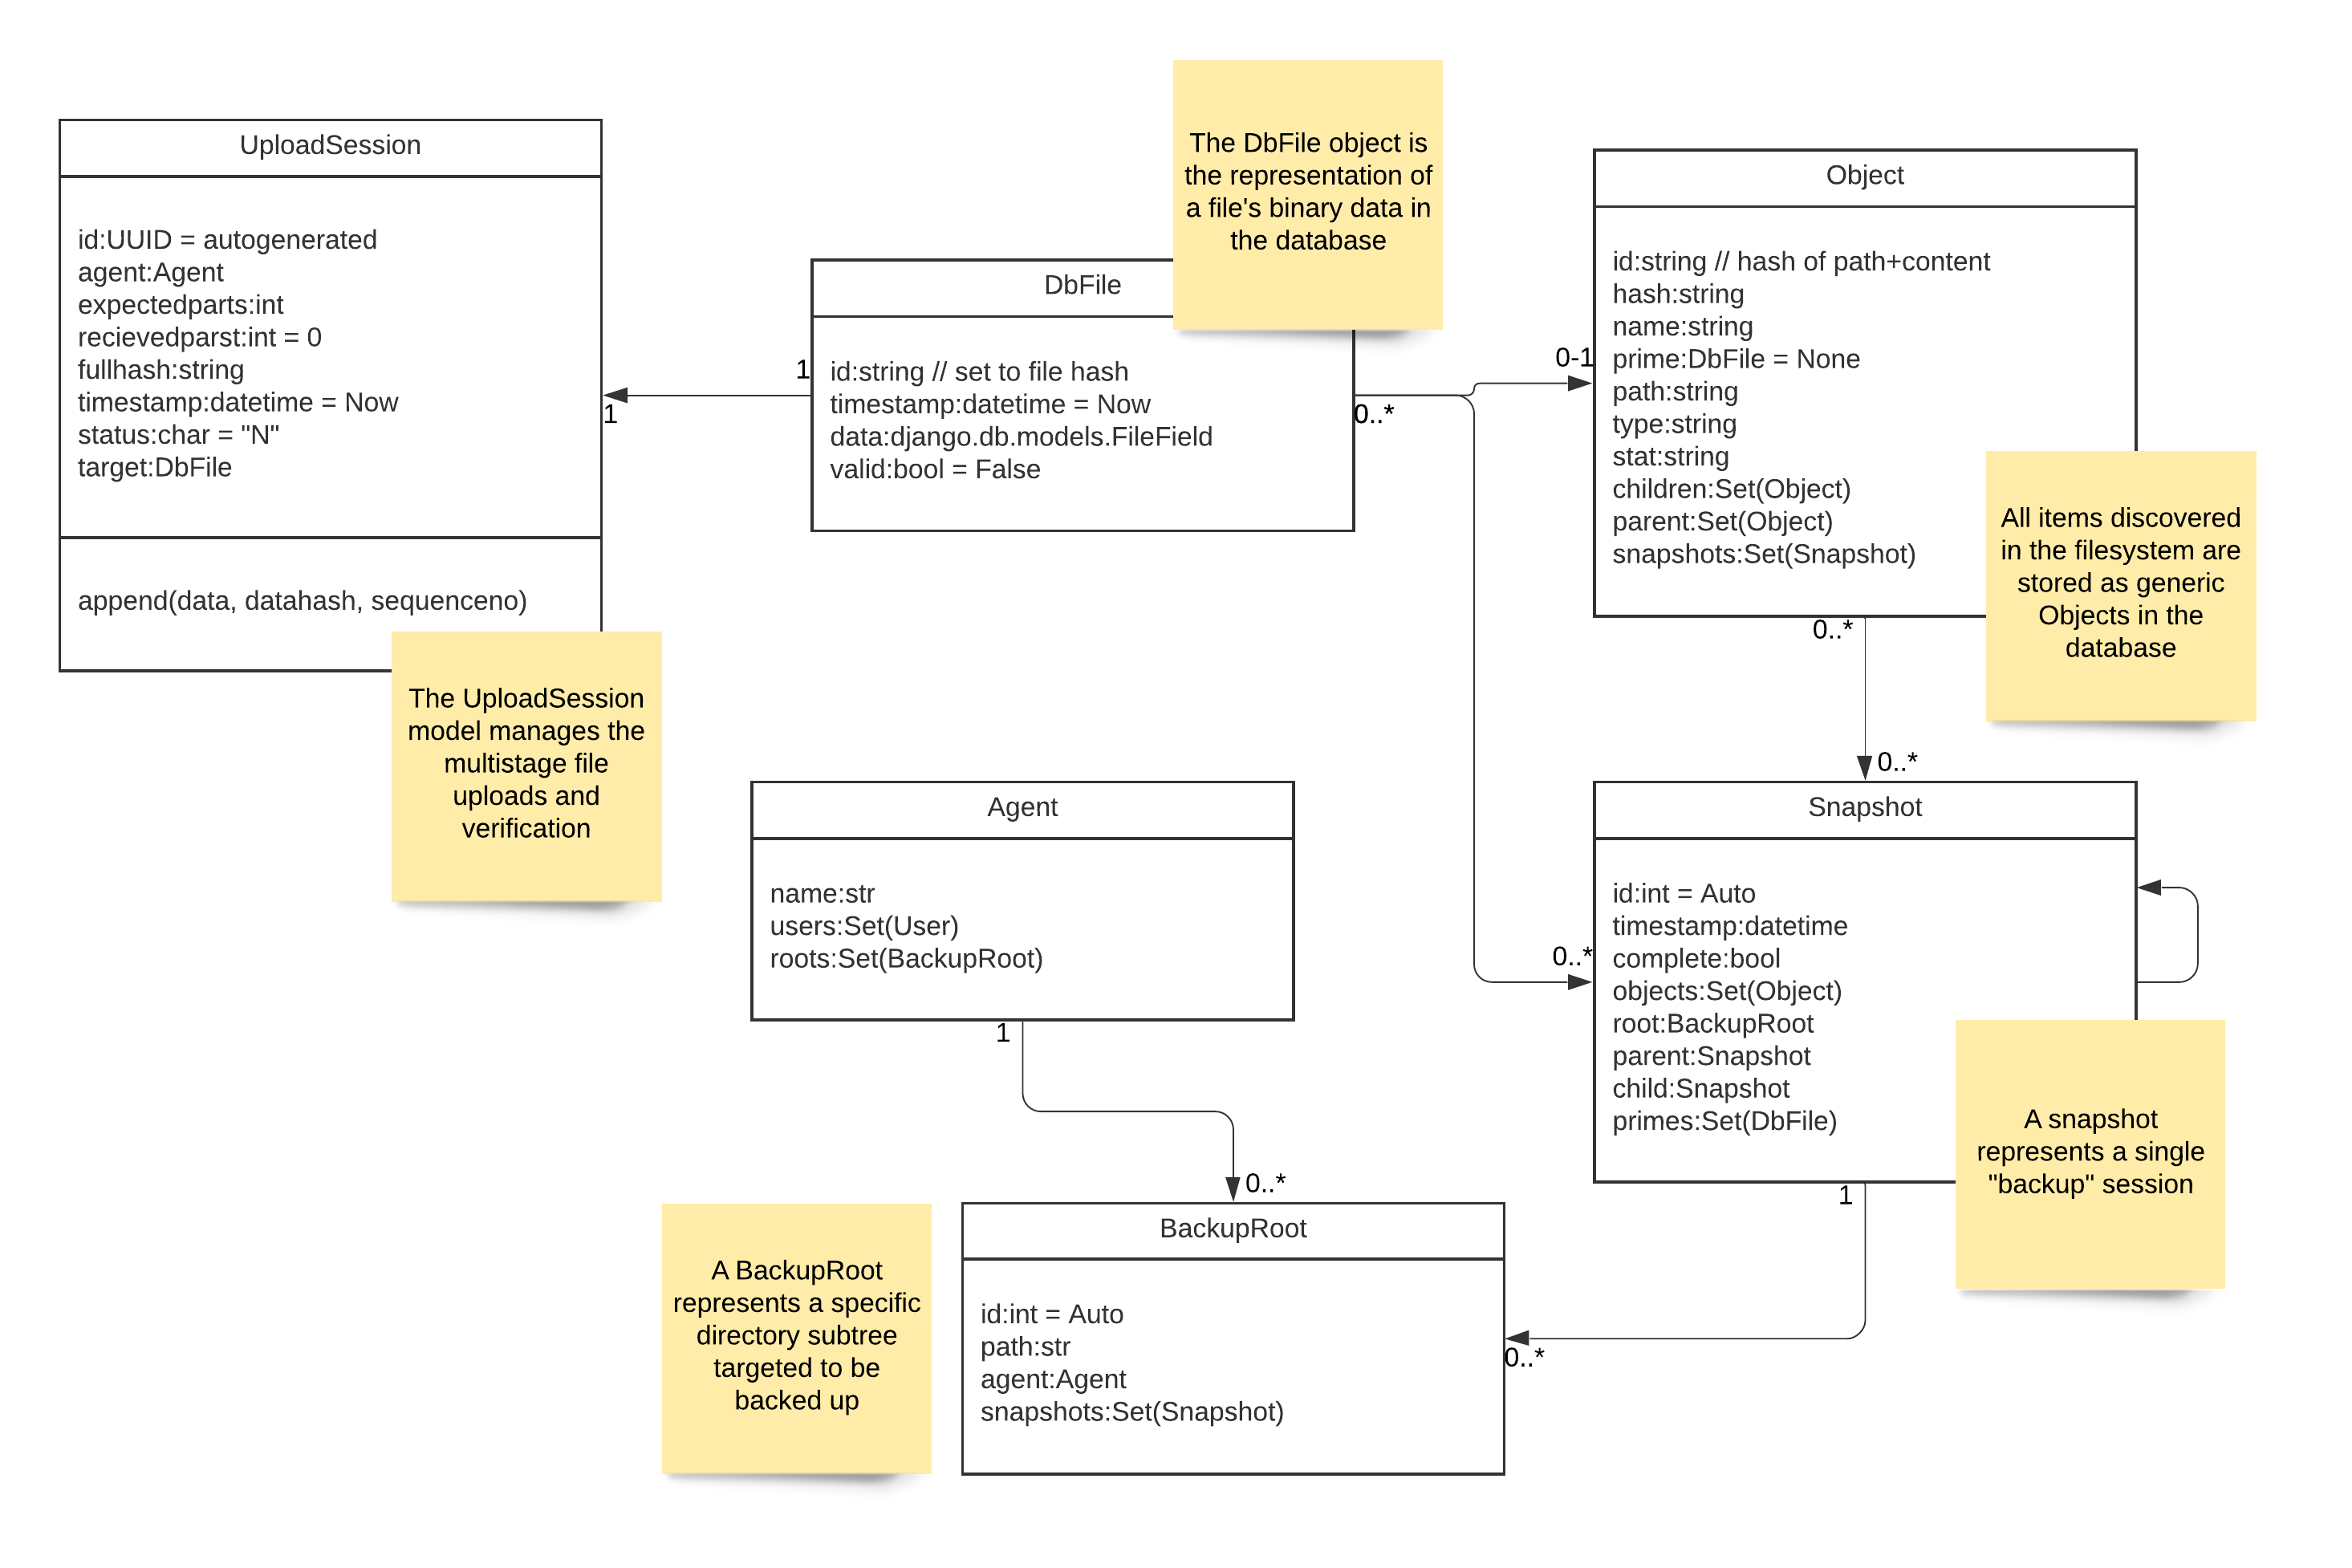
\includegraphics[width=0.82\paperwidth]{img/serverfileuml}
	\caption{UML of Django ORM models used to manage backup data}
	\label{serverdjangofileuml}
\end{figure}

File data is stored wrapped within a \texttt{django.orm.models.FileField} attached to the DbFile 
object and stored on the filesystem of the CoStor server at a location defined by the config file,
with the filename being the object's ID.

\section{Management UI}

This user interface provides access to all day to day configuration tasks, shows telemetry for
all clients and replication status and allows an administrator to browse the directory tree of
backup snapshots for any agent enrolled against the server.

\subsection{Monitoring}

Below is a wireframe of the monitoring view for CoStor clients enrolled against the server. This
view allows an administrator to check at a glance whether agents have checked in recently, total
and individual disk usage and any recent errors. It also shows the result of recent automatic 
maintenance tasks.

\subsection{Data browser}

Mockup of data browser UI

\section{Restoring backups}
\label{sec:restoringbackups}

\todo[inline]{Restoration has not yet been fully implemented}

There are two main procedures for restoring backups from CoStor, depending on whether the data
is stored on the local server (a direct restore) or whether data is being restored from 
geo-replicated copies of the database, in the event the site's own instance has failed.

\subsection{Direct (local) restore}

These are the most straightforward of restores, the administrator simply has to find a directory
or object within the data browser interface for an agent and snapshot within the web UI for their 
site's local instance of CoStor server, before requesting a restore package be generated. CoStor 
then re-builds the original directory tree selected from database objects and creates an archive
of the backup which can be downloaded and restored manually.

\subsection{Remote (disaster recovery) restore}

In the event that the instance of CoStor has failed for the site that is being backed up, there
are additional steps.

\begin{enumerate}
	\item As all metadata for replicated sites is encrypted, a valid master decryption key must
	be provided to the server being used to restore a backup. This is checked against the master
	federation database, which is replicated to all servers within the group.
	\item The server then identifies which CoStor servers contain copies of the metadata 
	databases for the requested site (using the global master federation database), and requests
	that metadata be replicated to itself if the data is not already available locally.
	\item Finally, the server decrypts the replicated metadata for the requested agent and 
	snapshot, allowing the administrator to generate a restoration archive using the same
	method for a local restore: browsing the directory tree and selecting required sub-trees
	to be restored. File "primes" or binary data blocks are decrypted on the fly before being 
	written to the restoration archive.
\end{enumerate}

\subsection{Local (disaster recovery with new server) restore}

In the event that the hardware running CoStor has to be replaced, it is possible to replicate
all data for that site back to the new server from the replicated copies across other sites.

\begin{enumerate}
	\item The new instance should be configured with the same ID, encryption key and access 
	token as the original server, to re-enroll it into the network. The master federation 
	database will then be replicated to this new server.
	\item The new (replacement) server can then request that all replicated data from its site
	is returned to its local storage, and will decrypt each package as it arrives to rebuild
	the server's original state.
	\item Once all data has been restored to the server, the restoration continue as outlined
	in the direct (local) restore procedure.
\end{enumerate}

\section{Automated maintenance tasks}

To ensure that the CoStor server can run for extended periods of time without requiring regular
maintenance, a series of day-to-day tasks are automated. These include:

\begin{itemize}
	\item \textbf{Purging of old data}:
	CoStor will automatically purge old snapshots and orphaned metadata entries once the retention
	window set by the administrator has expired.
	
	\item \textbf{Disk space monitoring}:
	Should the disk space become limited on the host, an email will be sent to the administrator
	to notify them that this is the case before backups fail.
	
	\item \textbf{Hard drive SMART testing}:
	CoStor can be configured to automatically run periodic SMART tests on hard drives within the 
	server, and notify administrators in the event of an anticipated failure. This very simply runs
	the \texttt{smartctl}\footnote{\url{https://linux.die.net/man/8/smartctl}} command and parses 
	the command line response.
	
	\item \textbf{Replication configuration updates}:
	CoStor is clever enough to automatically change replication targets, should any of its currently 
	selected targets become unavailable for whatever reason (such as lack of disk space or hardware 
	failure).
	
	\item \textbf{Offline client notifications}:
	If an instance of the client hasn't completed a backup in a defined period of time, the 
	administrator will be notified to allow them to investigate.
\end{itemize}

These tasks are run on a fixed schedule, prior to replication tasks running, in a Celery task
runner.

\chapter{Multi-site replication}

\todo[inline]{The mechanics for this are currently still being prototyped.}

The data to manage multi-site restores is stored in a globally replicated database, which 
contains information such as the replication status of all snapshot directory trees and file 
"prime" objects, anonymised agent ID to site mappings, and synchronisation job objects to track
when and to where objects are replicated.

Each site manages its own replications, and responds to replication requests from other servers
within the network. All objects are identified globally by the hash of their contents, and 
database objects are replicated as encrypted JSON documents. File "primes" are transferred using
the large file upload protocol used by the clients (outlined in Figure \ref{fig:lfileupload})

The overall goal of the replication system is to ensure there are at least two redundant, offsite
copies of all data. This is performed by selecting replication targets randomly, weighted by 
free disk space, and by incrementally scheduling the replication tasks during a configured
maintenance window (normally overnight when the network is quiet).

\section{Data distribution and sharding}

Each server will choose two sites to distribute its data across to. This means that each instance
of CoStor will be holding the backup data of its own site, plus compressed copies of two other
sites backups.

\section{Replication management database}

To allow all federated instances of CoStor to collaborate on managing replication tasks, and to
enable restoration from federated data even if the master database for that site is unavailable 
(in the event of a server failure), the replication data is synchronised across all servers.

All operations on these database tables are wrapped such that an API request is made to all other
servers to update them immediately. Additionally, before a replication task commences, a full
sync is requested to ensure that all servers contain all objects. To allow the servers to easily
verify data integrity across nodes, all entries in this database have a UUID and are write only. 
When a sync is triggered, the server sends a request to all other CoStor servers with the full 
list of object IDs. If any IDs are missing, each server requests copies of these. If any server
finds that it has an object with an ID that isn't in the list, it can assume that object has been 
deleted and will purge it from its own copy of the database.

This database contains information such as which backup Objects and file "primes" 
(Figure \ref{serverdjangofileuml}) have been replicated to which locations, current status of all
nodes, and basic information on which sites own which agents and snapshots. This database 
\textbf{must} contain all the information needed to initiate a restore in the event of a remote 
disaster recovery restoration (Section \ref{sec:restoringbackups}). As only the server to
be modifying data relating to a site is the server located in that site, there is no risk of 
requests interfering with each other.

As almost every object in CoStor is referenced by a unique and anonymous ID, there is minimal 
risk in sharing this data with other servers.

\section{Securely synchronising data}

\todo[inline]{The following concept relies heavily on file "primes" being stored in CoStor with
convergent encryption\cite{macbac-lisa}, for cross-site deduplication, which has not yet been 
implemented in the core CoStor client and server applications.}

\large \textit{"How do we share data across sites without risking breach of confidentiality?"}
\normalsize

To enable the backup databases to be replicated securely, replicated data is stored using a modified
subset of the standard database objects used by the local backups (Figure~\ref{serverdjangofileuml}).

The actual DbFile objects do not require changing, as the data is already stored encrypted, and thanks
to the use of convergent encryption, the ID (or hash) of all of these objects is already the same as
those stored from the target server's local backups. The Object class is modified such that the name,
path and stat fields are stored as encrypted strings, but as the IDs, agent and snapshot IDs are unique
across sites, as well as being anonymous, these foreign keys can continue to be used.

\section{Efficiently transferring data}

We also need a way to transfer that data between hosts. As we already have serialisers for the 
database models thanks to the Django Rest Framework, it makes sense to re-use these to transfer 
database objects as JSON data. This also allows us to combine multiple entries into one large
request, as an entire snapshot's worth of data is still fairly small.

For file primes, if they are not already present on the target server, we can give these a quick bit
of compression using something fast like LZ4\footnote{\url{https://github.com/lz4/lz4}} to compress
each object before transmitting it using a modified version of the large file protocol utilised by
the client, described in Figure~\ref{fig:lfileupload}. These can then be decompressed and added to that
site's local DbFile store, where they may come in useful for local backups as well.

\chapter{Testing and evaluation}

Beyond being a cheap, self-hosted option to cloud backup, CoStor has two main goals:

\section{Being a reliable backup solution}

Testing for actual backup performance, and fault-tolerance, using a combination of real-world data
such as test installs of operating systems, and backups of my various machines!

\section{Being easy to use and manage}

Testing the web management panel and installation process using user studies.

% use the following and \cite{} as above if you use BibTeX
% otherwise generate bibtem entries
\bibliographystyle{IEEEtran}
\bibliography{costor-references.bib}

\end{document}
